\documentclass[10pt,letterpaper,conference]{IEEEtran}

\usepackage{cite}
\usepackage{amsmath}
\usepackage{comment}
%\usepackage{times}
\usepackage{epsfig}
\usepackage{url}
\usepackage{multirow}

%\textheight 688pt

\begin{document}
\title{Design Implications of Multi-Level Cell ReRAM-based Memory Hierarchies\vspace{-10pt}}
%\author{Cong Xu\dag, Dimin Niu\dag\ddag, Norman P. Jouppi\ddag, and Yuan Xie\dag\\
%\dag Department of Computer Science and Engineering, Pennsylvania State University\\
%\ddag Intelligent Infrastructure Lab, Hewlett-Packard Labs\vspace{-15pt}}

\maketitle

\begin{abstract}
Resistive Random Access Memory (ReRAM) recently has been a promising candidate for next-generational memory technology when there is a foreseeable growing demand for large capacity memory in future computer architecture. The capability of storing multiple bits in a single ReRAM cell further improves the memory density and reduces cost per bit significantly. Multi-step write-and-verify scheme is required in multi-level cell (MLC) ReRAM programming due to the existence of all sorts of variations. The traditional programming approaches have the drawbacks of either long average write latency or possibility of retention failure in some programmed states. In this work, we proposed two sets of programming approaches targeted at reducing write latency/energy and improving the memory reliability separately. Hardware designer can adopt either set of programming approach based on the requirement of memory sub-system specifications in the memory hierarchies. 
\end{abstract} 
\section{Introduction} \label{sec:intro}

Memory hierarchy design~\cite{CACTI51} is becoming one of the most important factors in modern computer systems. The importance of the memory hierarchy increases with the advances in performance of the microprocessors. DRAM has been the common memory technology for main memory while maintaining the capacitor is becoming more and more difficult with the scaling of the feature size of the DRAM process. NAND flash has been widely adopted in storage system such as solid-state disk (SSD) and USB drivers. But there are multiple issues associated with the scaling of NAND flash including floating gate interference, charge loss tolerance and small cell current and coupling ratio. Emerging memory technologies usually have the advantages of high density, non-volatility, zero standby power from memory cells. Among these memory technologies, Phase-change Random Access Memory (PCRAM) and ReRAM have demonstrated excellent scalability beyond 10nm technology node[??] and both of them can be built in crosspoint array structure[??]. Thus PCRAM and ReRAM are being explored as potential alternatives of cost-sensitive DRAM and/or NAND flash. Spin-torque transfer Random Access Memory (STTRAM) has unlimited write endurance while offers 3X-4X more density than SRAM, and is considered as the replacement of on-chip caches[??].

ReRAM have balanced metrics in many aspects, making it a good fit for different levels in memory hierarchies. Compared to PCRAM, ReRAM has much better write properties and slightly more endurance in single-level cell (SLC) operation. It reduces the SET/RESET current from hundreds of microamps (for PCRAM) to tens of microamps and also decrease the single SET/RESET pulse width from at least tens of nanoseconds (for PCRAM) to only a few nanoseconds. Combing the savings in both write current and write time, the switching energy per cell of ReRAM is less than one percent of that of PCRAM, thus solving the well-known power-hungry issue for PCRAM prototypes. Moreover, more than $10^{12}$ write cycles has been reported in several SLC ReRAM technologies [??] while the typical endurance of current PCRAM technology is less than $10^{10}$. Compared to STTRAM, ReRAM has much better read properties and smaller cell size. The large on/off ratio (>100 for many ReRAM technologies) makes it easier to sense the ReRAM resistance difference between high resistance state (HRS) and low resistance state (LRS), considering the typical resistance ratio of STTRAM is smaller than 3.

Projected as a low cost-per-bit memory technology, ReRAM has several features in improving memory density. First, ReRAM has the capability of building cross-point memory arrays, leading a memory cell of only $4F^2$. The array size of cross-point structure is a critical design parameter which has strong impact on the overall footprint of ReRAM prototype [?cong's date?]. It was found that the nonlinearity of the cell size is the key factor in reducing sneak leakage current and thus determining the maximum array size. Some ReRAM technologies have good nonlinearity by nature [?unity, hp?] while most ReRAM technologies need a diode-like device in serial with the ReRAM cell to get enough effective nonlinearity. Fortunately, there materials with required properties such as enough driving current density, CMOS-compatability, scalability have been widely explored [??] and are better engineered to incorporate in "1D1R" structure. Second, multi-layered crosspoint structure can be built to further reduce the memory cell size to $4F^2//n$, where n is the number of stacking crosspoint layers. 4-layered crosspoint ReRAM prototypes have already been demonstrated with reliable read and write operations. However, multi-layer stacking extends the effective array size in the vertical dimension while the maximum array size is still constrained by the nonlinearity, wire resistance, Third, many ReRAM material systems,
such as CuOx[??], TiOx [??], HfOx [??], WOx [??], and TaOx [??], were reported to be capable of MLC operation. Table ? summarizes the current demonstrated MLC ReRAM metrics in different ReRAM technologies. There are many endurance/speed/power trade-offs of MLC operations in different ReRAM material systems. For example, compared to $T_iO_x$-based ReRAM, $T_aO_x$-based ReRAM has better endurance but needs large RESET voltage (>5V). MLC offers another opportunity to improve ReRAM density and is potentially a orthogonal solution to crosspoint structure. But like the choice of multi-layer stacking, MLC degrades the read and write margin in crosspoint array and needs better cell-level characteristics or circuit-level design tricks to maintain the same array size.

\begin{table}[t]
\centering
\caption{Characteristics of MLC metrics in ReRAM technologies}
\vspace{-5pt}
\label{tb:0t1r}
\begin{tabular}{ l | c | c | c | c | c}
\hline\hline
Material System & $T_iO_x$ & $T_aO_x$ & $H_fO_x$ & $WO_x$ & $C_uO_x$\\
\hline
MLC levels & 5 & 4 & 5 & 8 & 5\\
\hline
$R_{off}$/$R_{on}$& $>1000$ & $>1000$ & $>100$ & $>10$ & $>100$\\
\hline
MLC endurance  & $>10^6$ & $>10^7$ & $>10^5$ & $>10^4$ & -\\

\hline\hline
\end{tabular}
\vspace{-10pt}
\end{table}

Multi-step write-and-verify scheme is required in MLC ReRAM programming because there exists both device-to-device variation due to process variations and cycle-to-cycle variation due to stochastic switching mechanism. The desired resistance states can be achieved in two opposite directions. We can start from the HRS state and get the intermediate LRS resistance by controlling the amplitude of the SET current. This is due to due to the modulation of the diameter or the number of conductive filaments (CFs). Or we can start from the LRS state and get the intermediate HRS resitance by controlling the amplitude of the RESET voltage. This is due to the modulation of the ruptured CF length.




\section{Preliminaries} \label{sec:preliminary}

In this section, we will describe the background of ReRAM technology, switching mechanism of the device and characteristics of retention failure observed in some ReRAM resistance states.

\begin{figure}[t]
\centering
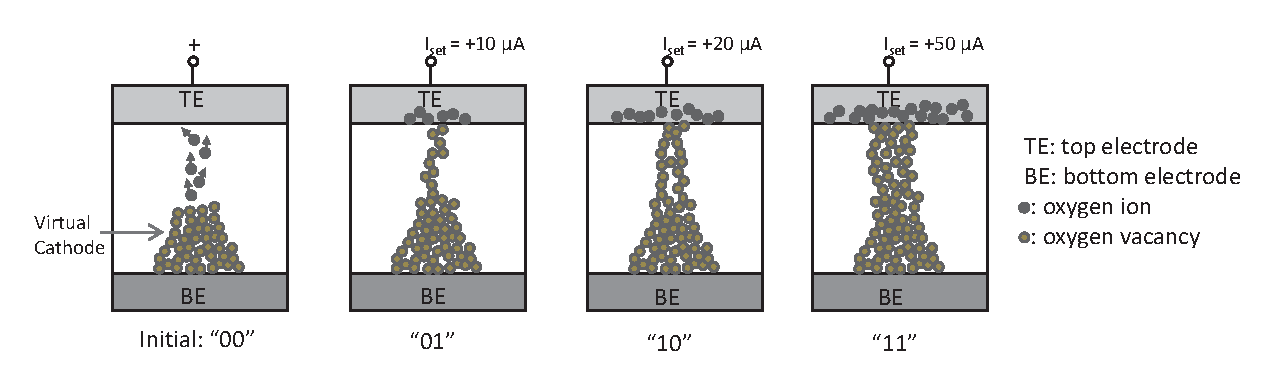
\includegraphics[width=0.48\textwidth]{fig/h2lview}
\vspace{-10pt}
\caption{Conceptual view of H2L programming.}
\label{fig:h2l}
\vspace{7pt}
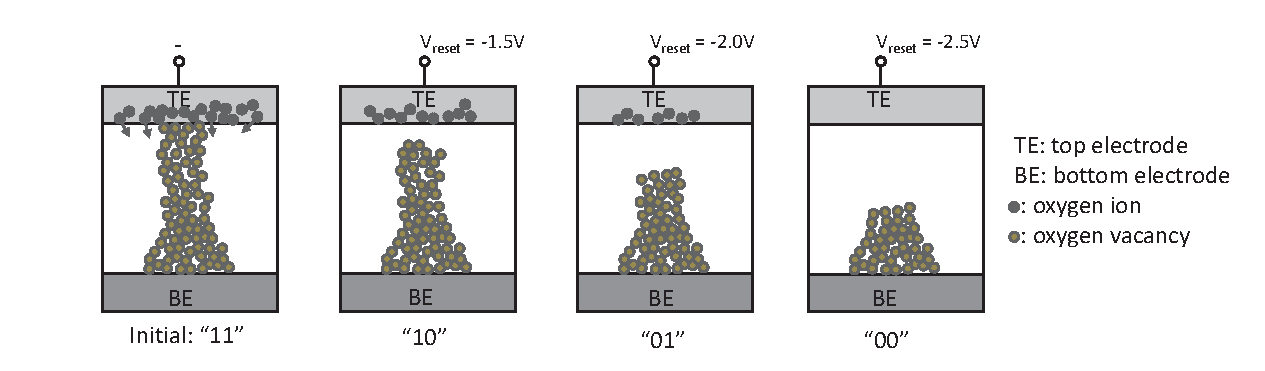
\includegraphics[width=0.48\textwidth]{fig/l2hview}
\vspace{-10pt}
\caption{Conceptual view of L2H programming.}
\label{fig:l2h}
\end{figure}

\subsection{Background of ReRAM technology}
The basic structure of a ReRAM cell is a metal layer sandwiched between two metal electrodes, called metal-insulator-metal (MIM) structure. The switching from HRS to LRS is defined as SET operation while the opposite process is RESET operation. The switching modes of ReRAM can be broadly classified into two modes: unipolar and bipolar. Unipolar means SET/RESET operation only depends the amplitude of the applied voltage/current but not on the polarity. Bipolar means SET and RESET occurs at different polarity. The switching mechanism and characteristics does not only depend on the choice of metal oxide layer but also the electrode materials and their interfacial properties. Some of promising oxide materials include $H_fO_x$, $T_iO_x$, $T_aO_x$, $N_iO_x$. An extremely fast switching ($<0.3ns$) has been reported for $H_fO_x$-based ReRAM [?ITRI?] and its endurance bar was recently raised to $10^{12}$ [??]. $T_aO_x$-based ReRAM has also demonstrated nanosecond switching [??] with endurance greater than $10^{12}$ [??]. $T_iO_x$ was interesting because of its intrinsic nonlinearity provides a low-cost solution for building crosspoint structure[?HP?]. Among all the ReRAM technologies, $H_fO_x$ seems to be have balanced metrics in switching time, switching energy, resistance ratio and endurance. Later in our case studies we will use $H_fO_x$-based ReRAM as an example. However, the discussion and solution we will have can be broadly applied for most ReRAM technologies with MLC capability.

\begin{figure}[t]
\centering
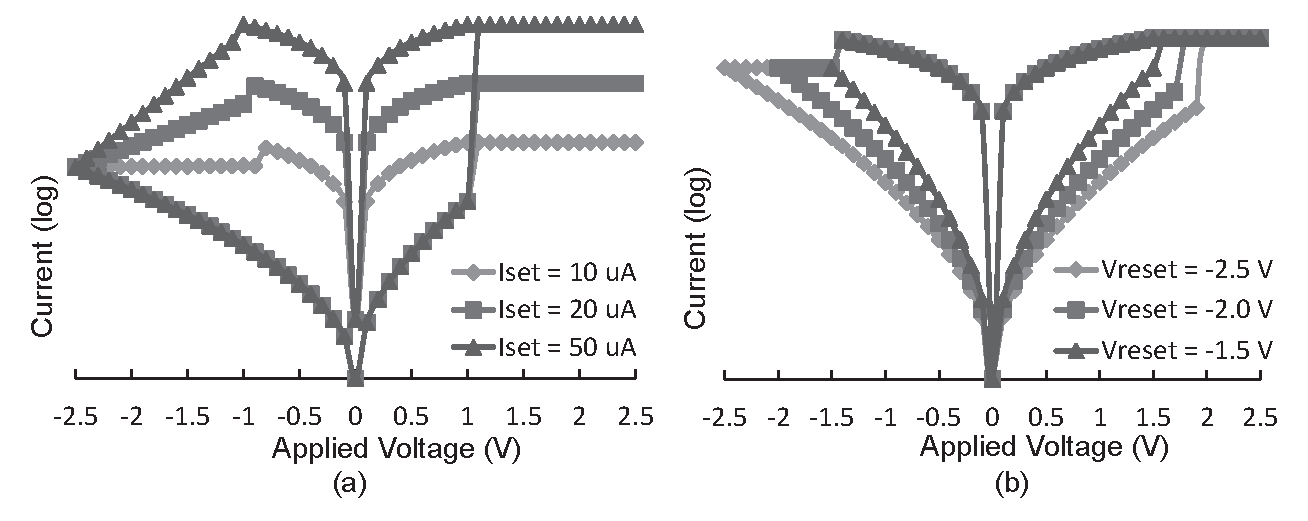
\includegraphics[width=0.48\textwidth]{fig/i-v}
\vspace{-10pt}
\caption{I-V curves demonstrate MLC characteristics of (a) H2L programming and (b) L2H programming.}
\label{fig:memristor}
\vspace{-15pt}
\end{figure}

The triggering of switching behavior of ReRAM is closely related to the formation or rupture of so-called conductive filament (CF), which consists of oxygen filaments. Once a filament is created inside the metal oxide layer and connects top electrode with bottom electrode, electrons can hop through the CF resulting in a LRS of the cell. The strength of the CFs is determined by the diameter or the number of CFs. The stronger (larger or more number of) the CFs are formed, the lower resistance the LRS is. Similarly, the rupture of CFs disconnects two metal electrodes and create a HRS of the cell. The resistance of the HRS is roughly proportional to the rupture length of CFs. Figure ? illustrates the formation process of the CFs in a ReRAM cell and the controlling of CF strength by adjusting the amplitude of SET current. When a positive current passing through the cell, the oxygen atoms are knocked out of the lattice and become negative-charged oxygen ion. The oxygen ions will be drift towards the anode and leaving corresponding oxygen vacancies in the metal oxide layer. CFs are formed when enough oxygen vacancies were created and connected as a conductive path. As we can see from the figure, stronger CFs are formed when more SET current pass though the cell for the same amount of time. This is the fundamental reason that a ReRAM cell can be programmed into intermediate levels of LRS, enabling the feasibility of MLC. The programming approach is defined as H2L (HRS-to-LRS) programming. The completely opposite MLC programming direction is to vary the RESET voltage so that the rupture length of the CFs can be controlled, as seen in Figure ?. When a RESET voltage is applied cross the ReRAM cell in LRS, oxygen ions migrate back to the metal oxide layer and combine with oxygen vacancies. For unipolar ReRAM, this is primary due to Joule heating. For bipolar ReRAM, the migration of oxygen ions is assisted by both thermal diffusion and a reverse dielectric field. As the RESET voltage is ramped up, the HRS resistance is increased due to increased rupture length of the CFs. This process is defined as L2H (LRS-to-HRS) programming.

\begin{figure}[t]
\centering
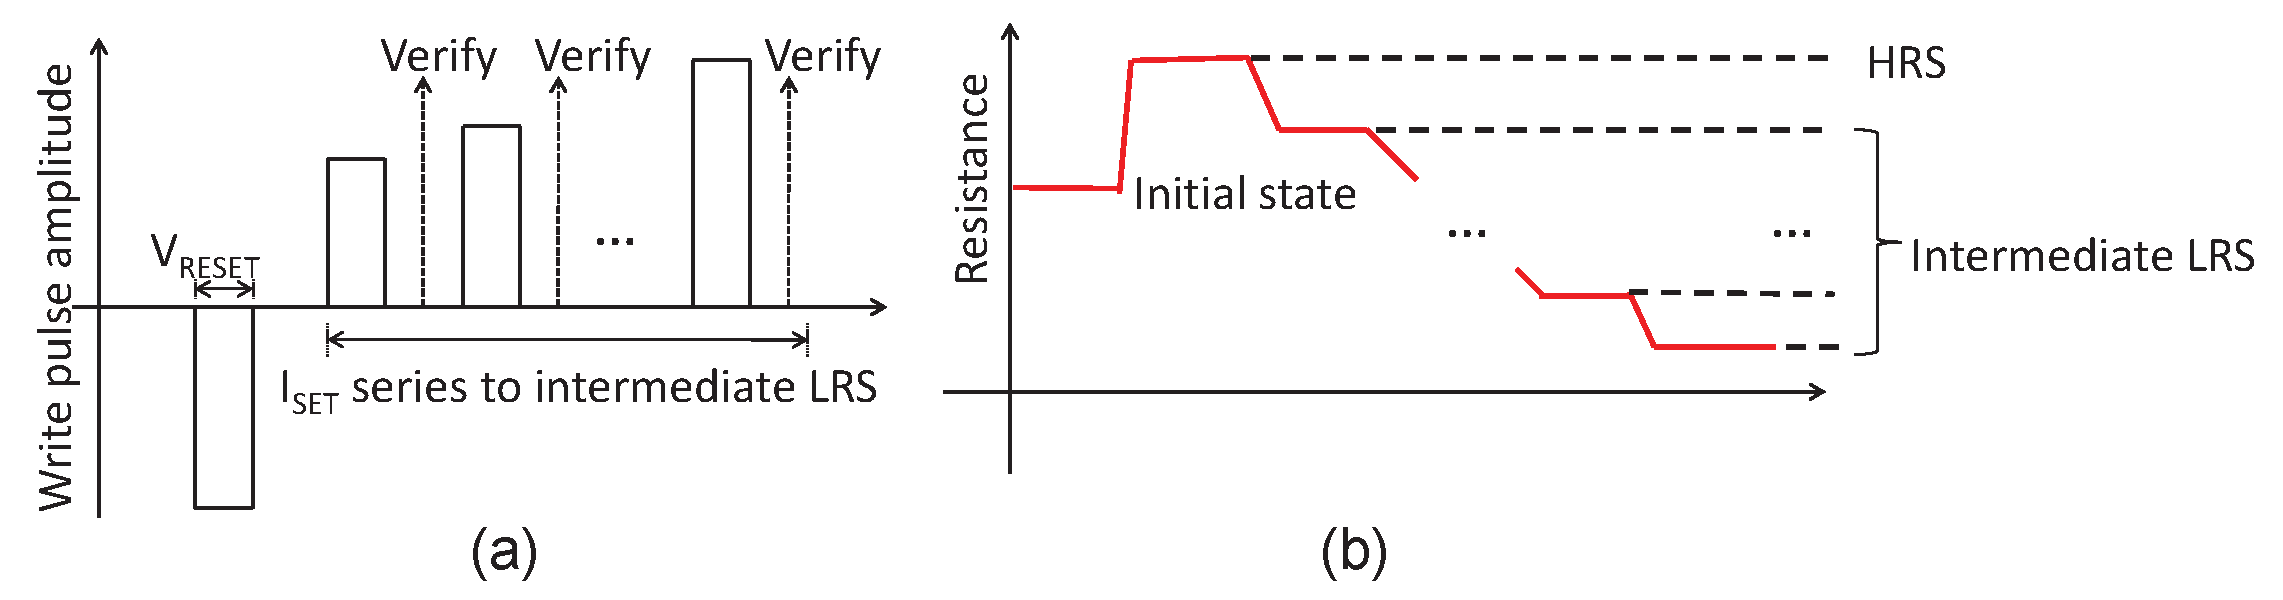
\includegraphics[width=0.48\textwidth]{fig/WandV}
\vspace{-10pt}
\caption{Write-and-verify scheme for H2L programming: (a) A RESET voltage is first applied and then SET current is ramped up; (b) The resistance change corresponding to applied pulse series.}
\label{fig:wv}
\vspace{-15pt}
\end{figure}

Multi-step write-and-verify (W\&V) scheme is required in MLC ReRAM programming due to the existence of  both device-to-device variation and cycle-to-cycle variation. The device-to-device variation (or spatial variation) sources mostly from process variations (PVs) in device geometries and material properties. The impact of PVs on ReRAM was studied in [?DiminDAC?]. Stochastic switching behavior is the unique characteristic of ReRAM technology because the generation and degeneration of oxygen vacancies are naturally probabilistic and nondeterministic even under the same environment (i.e. electric field, oxygen concentration). That essentially means for a particular ReRAM cell, the resistance after the same SET current or RESET voltage has been applied for the same amount of time is difference from cycle to cycle. Using multiple pulses or a ramped series of pulses and introduce verification after each pulse helps improve the cycle-to-cycle uniformity [?123,124?]. The programming methodologies we propose later are all based on write-and-verify scheme for practical MLC applications.

\subsection{MLC read operation}

\subsection{Impact of Retention Failure on MLC reliability}
 Superior to SRAM and DRAM based on charge storage, emerging NVMs such as ReRAM and STTRAM are immune to soft errors caused by particle strike. However, each NVM technology still has non-zero "soft" (or recoverable) failure probability. The soft error of STTRAM can be caused by thermal fluctuations [?guangyuICCD?] and the failure rate increases as the thermal stability factor is lowered by PVs. The soft error of PCRAM relies on both short-term and long-term resistance drift [?free-p?], causing a well-known reliability issue of MLC PCRAM. Unlike the gradual resistance drift in PCRAM, a sudden resistance transition may occur in a ReRAM cell[?Bin?]. The sudden transition from HRS to LRS is referred as a HRS retention failure while the opposite transition is referred as a LRS retention. The retention failure essentially share the same principle with normal switching behavior or ReRAM - formation and rupture of CFs. For example, HRS failure is due to the generation of oxygen vacancies by a thermal activation process, which is a random process and requires much more time than typical write operation. [?Bin?] concludes that for ReRAM with large SET current ($>500\mu A$), strong CFs are formed (SET) or ruptured (RESET). In that case only HRS retention failure is observed because ruptured CFs are more like to be reconstructed. In contrast, for ReRAM with small SET current ($<100\mu A$) [?Shimeng?], only LRS retention failure is observed because weak-formed CFs are more likely to be ruptured due to the random degeneration of oxygen vacancies in the CFs. The test results in [?JubongPark?] in confirms that there exists reverse linear dependence between LRS resistance and retention failure time: $t_{failure }\propto 1/R_{LRS}$. Therefore, we identify, for the first time, the reliability issue in MLC ReRAM applications: in H2L programming higher LRS resistance levels are associated with weak CFs and are vulnerable to LRS retention failure; in L2H programming most HRS resistance levels are with strong CFs and are vulnerable to HRS retention failure.

\section{Programming Methodologies} \label{sec:programming}

In this section we propose two programming methodologies targeted very differently. The fast MLC programming methodology is devised for ReRAM memory when performance is a very critical and seldom soft error can be tolerated. This assumption holds true for main memory in traditional memory hierarchy. DRAM-based main memory are usually designed with ECC to tackle particle-strike soft error. More importantly, most of the data in main memory does not have to be "stored" for a long time as either they will be updated frequently or they will be useless without future accesses. The reliable MLC programming methodology is more suitable for storage system where data integrity is extremely important. For example, the data in SSD or USB driver may need to be stored for years. Moreover, even microsecond-level write latency can be hidden by large block size in conventional NAND flash product, maintaining an acceptable bandwidth. We will use 3-bit MLC cell as illustrations in this section since 8-level stable states have been widely reported in experimental data for MLC ReRAM. We denote the three bits in a ReRAM cell as $D_2D_1D_0$ where $D_2$ is the most significant bit (MSB) and $D_0$ is the least significant bit (LSB). "111" denotes the lowest LRS resistance while "000" denotes the highest HRS resistance.

\subsection{Fast MLC programming methodology}

\begin{figure}[t]
\centering
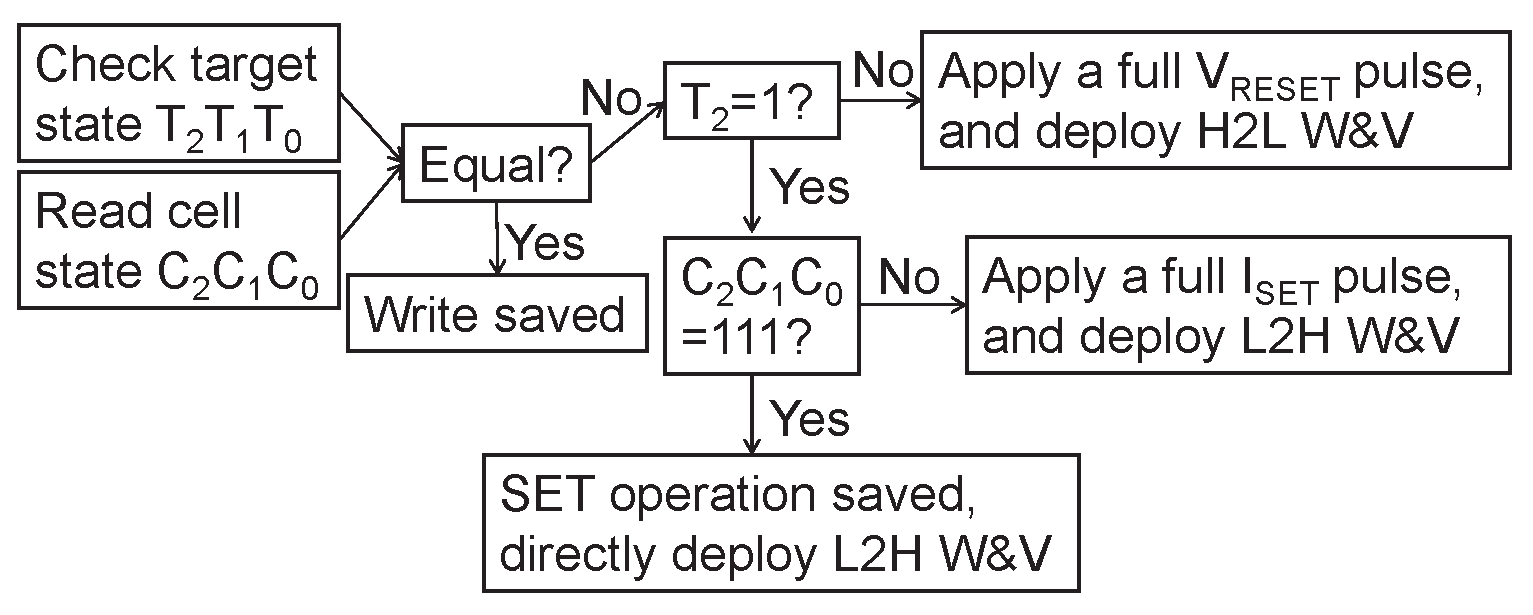
\includegraphics[width=0.48\textwidth]{fig/fastprog}
\vspace{-10pt}
\caption{Flowchart of fast programming methodology}
\label{fig:fastprog}
\vspace{-15pt}
\end{figure}

The goal of the fast MLC programming methodology is to reduce the average write latency by avoiding the states that require large number of iteration steps in either H2L or L2H programming. The flowchart of the proposed programming methodology is illustrated in Figure~\ref{fig:fastprog}. Before the actual programming starts, current state of the cell $C_2C_1C_0$ is first read out and compared with the target state $T_2T_1T_0$ to be programmed. If they are equal, the programming was skipped. Otherwise it is required to identify whether the target state easier to reach from HRS or LRS, which can be simply achieved by checking the MSB of the target state: $T_2=0$ means the target state is relative high resistance and may require smaller number of iteration steps in H2L programming. In that case, we apply a full RESET voltage across the cell and push it to the highest level of HRS and then deploy H2L programming. Note that read was first performed immediately after the full RESET operation and the first verification result indicates whether $T_2T_1T_0=000$ or not. If the $T_2=1$ then L2H programming may be preferred. Here an additional comparison is made to to save possible SET operation if original cell state is already in lowest level of LRS. If $C_2C_1C_0=111$ then we can begin L2H programming without a complete SET operation first, otherwise a full SET current pulse is applied on the cell first. So far, the first state-aware programming methodology is devised to achieve fast MLC programming speed by the speculation of both the target state and the original cell state. However, some programmed states by the fast programming methodology may be somewhat vulnerable to retention failure. For example, if $T_2T_1T_0=110$ the programmed state is achieved by slightly rupturing the strongly formed CFs and LRS retention failure is likely to occur in the cell. In contrast, if $T_2T_1T_0=001$ then weak CFs are reconstructed from HRS and HRS retention failure is likely to occur in the cell. Fortunately, the probability of retention failure under normal operation temperature of ReRAM is very small (smaller than the probability of DRAM soft error[??]). Therefore, the programming methodology can be widely adopted in MLC ReRAM application except for the scenario where the requirement of data retention is extremely restricted. Hence the second MLC programming methodology with excellent reliability is also proposed.

\subsection{Reliable MLC programming methodology}
\begin{figure}[t]
\centering
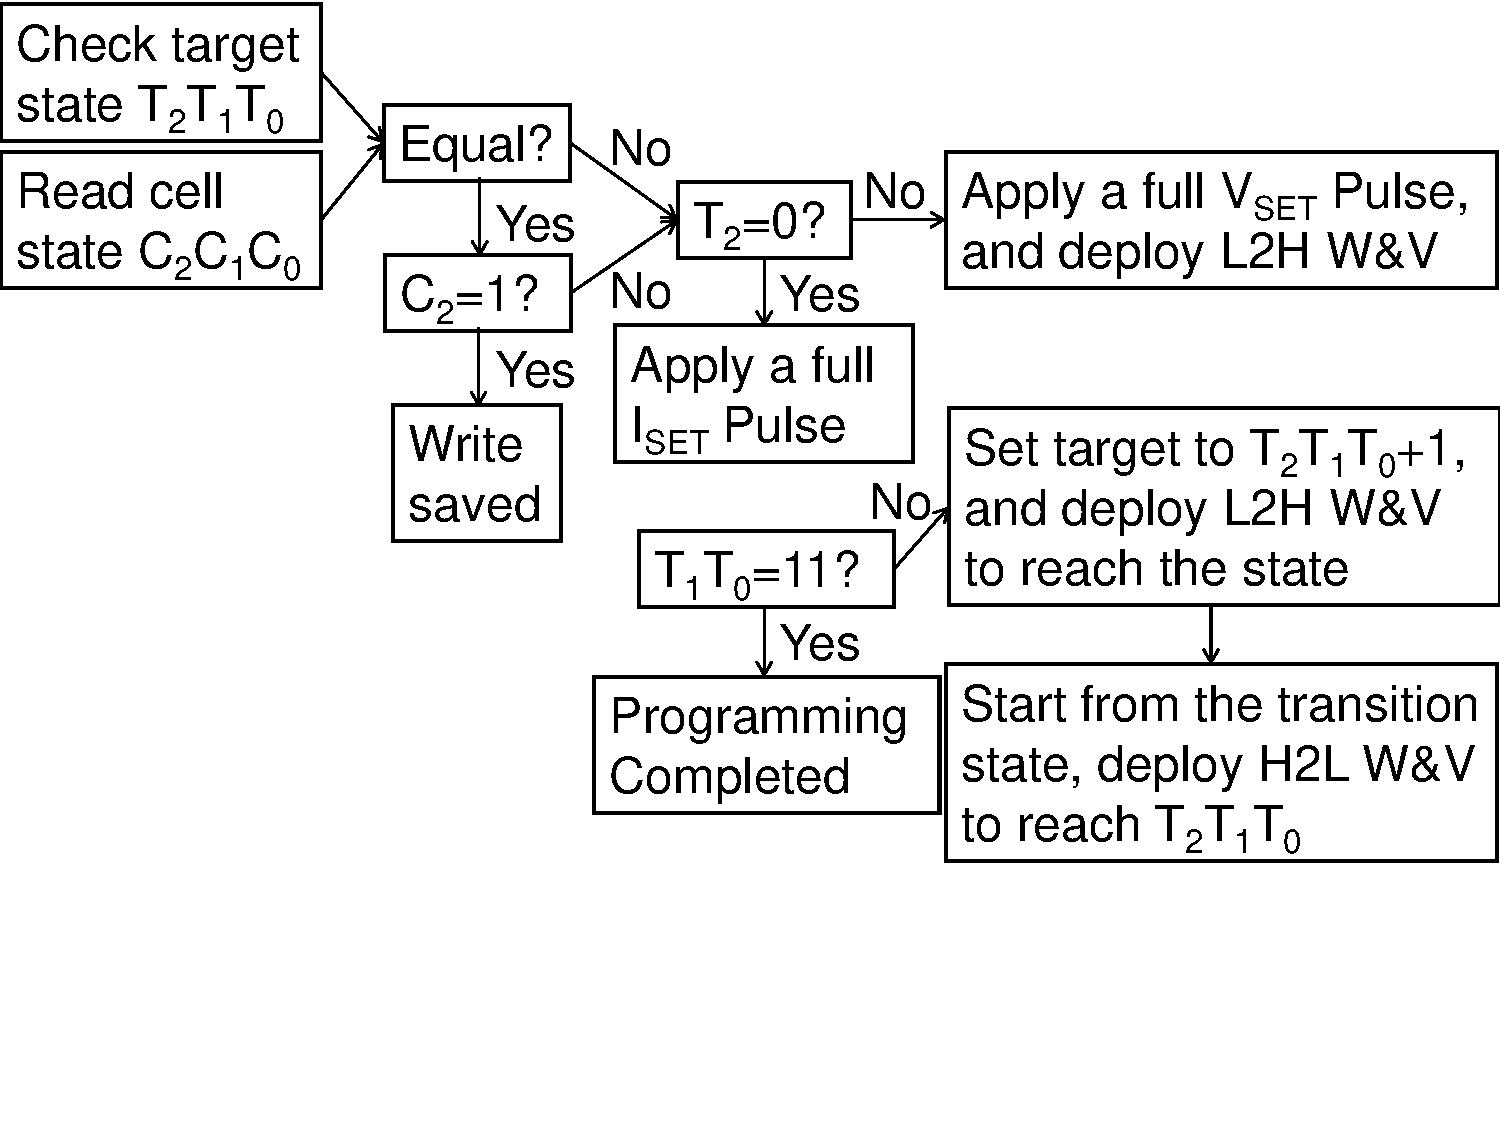
\includegraphics[width=0.48\textwidth]{fig/reliableprog}
\vspace{-10pt}
\caption{Flowchart of reliable programming methodology}
\label{fig:reliableprog}
\vspace{-15pt}
\end{figure}

The goal of the reliable MLC programming methodology is to meet the retention requirement (i.e. $>$years) of the programmed states by associating LRS with constructed strong CFs and HRS with ruptured weak CFs. 


\section{Peripheral circuitry design} \label{sec:peripheral}







\section{Experimental Results} \label{sec:experiment}







\section{Conclusion} \label{sec:conclusion}








\bibliographystyle{IEEEtran}
\bibliography{bib/cacti,bib/mram,bib/others,bib/pcm,bib/reram}

\end{document} 